\section{Métricas de evaluación}
\label{sec:metricas_evaluacion}

Antes de entrar a hablar de los modelos, vamos a ver qué métricas de evaluación usaremos para evaluarlos, ya que son la pieza clave para entender qué tan bien está funcionando un modelo concreto. Métricas de evaluación hay muchas, e incluso distintas según distintos problemas (regresión, clasificación, etc.). Las principales y más conocidas son la exactitud (\textit{accuracy}), f1, y Error Cuadrático Medio (RMSE), aunque hay muchas más como hemos mencionado. Vamos a listar todas las métricas que usamos, qué es lo que evalúan y en qué modelos las usamos (ya que algunas son tan importantes que se usan en casi todos los modelos). Es importante mencionar que, ya que nuestro problema es de clasificación, no usaremos algunas métricas de regresión como el RMSE, pues no podemos calcularlas ni tiene sentido. \\

\subsubsection*{Matriz de confusión}

Vamos a introducir también la matriz de confusión y el concepto de aciertos y fallos, ya que es fundamental para entender mejor las métricas. Un modelo puede hacer dos cosas, acertar y fallar, y, a su vez, los aciertos y los fallos pueden deberse a que la instancia fuera negativa y positiva. Con esto tenemos los siguientes conceptos:

\begin{itemize}
	\item \textbf{Verdaderos Positivos (VP)}: Insancias positivas predichas como positivas.
	\item \textbf{Verdaderos Negativos (VN)}: Insancias negativas predichas como negativas.
	\item \textbf{Falsos Positivos (FP)}: Instancias negativas predichas como positivas. También llamado Error tipo I.
	\item \textbf{Falsos Negativos (FN)}: Instancias positivas predichas como negativas. También llamado Error tipo II.
\end{itemize}

Las matrices de confusión toman esos cuatro valores y los distribuyen en: eje y los valores reales, eje x los valores predichos y se forma una matriz N x N, siendo N el número de clases que definamos. En nuestro caso, y en la mayoría de casos, se da una matriz 2 x 2, como se ve en la \nameref{fig:matriz_confusion}. También es importante entender que la diagonal principal siempre guarda los valores verdaderos (los aciertos de predicción). Con la figura queremos ilustrar cómo se ve una matriz de confusión 2 x 2. Normalmente se pone la clase negativa arriba/a la izquierda de la clase positiva, aunque podrían estar al revés, pero siempre manteniendo lo que comentamos de la diagonal principal.

\begin{figure}
	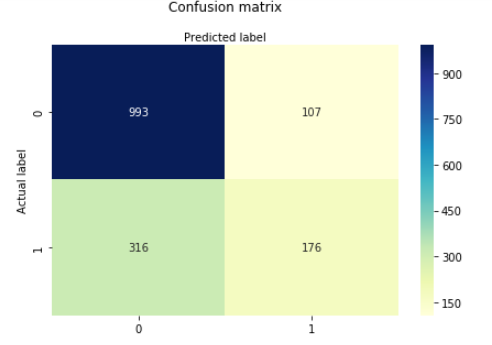
\includegraphics[scale=0.75]{imagenes/matriz_confusion.png}
	\caption{Ejemplo de matriz de confusión.}
	\label{fig:matriz_confusion}
\end{figure}

\subsubsection*{Métricas usadas}

Veamos entonces con lo que ya sabemos qué métricas usamos y qué miden.

\begin{itemize}
	\item \textbf{Exactitud (\textit{accuracy})}: Mide la proporción total de predicciones correctas (tanto positivas como negativas) sobre el total de casos. Es útil cuando las clases están balanceadas, pero puede ser engañosa si hay un desbalance (ej. 95\% de una clase y 5\% de otra, predecir siempre la mayoritaria daría un 95\% de accuracy). Su fórmula es: $\frac{VP + VN}{VP + VN + FP + FN}$. Lo usamos en Random Forest, LightGBM, SVM, Wav2Vec2, ...
	
	\item \textbf{Precisión}: Mide la relación de las clases predichas como positivas frente al total de valores reales positivos. Es una métrica que se enfoca en controlar los Falsos Positivos (FP). Es útil cuando el costo de un FP es alto (por ejemplo, marcar un correo legítimo como spam). Su fórmula es: $\frac{VP}{VP + FP}$. Podría calcularse la precisión para la clase negativa también. Lo usamos en Random Forest, LightGBM, SVM, ...
	
	\item \textbf{Exhaustividad (\textit{recall})}: Mide la cantidad de valores positivos que el modelo logró predecir correctamente. Es una métrica que se enfoca en minimizar los Falsos Negativos (FN). Es útil cuando el costo de un FN es alto (por ejemplo, no detectar una enfermedad grave). Su fórmula es: $\frac{VP}{VP + FN}$. Podría calcularse el recall de la clase negativa también. Lo usamos en Random Forest, LightGBM, SVM, ...
	
	\item \textbf{F1-Score}: Es la media armónica entre la Precisión y el Recall. Busca un equilibrio entre ambas métricas. Es una métrica más robusta que la Accuracy cuando hay clases desbalanceadas, ya que penaliza los extremos (una precisión alta con recall bajo, o viceversa). Es útil cuando quieres una sola métrica que resuma el rendimiento en la clase positiva. Su fórmula es: $2 \cdot \frac{\text{Precision} \cdot \text{Recall}}{\text{Precision} + \text{Recall}}$. Lo usamos en Random Forest, LightGBM, SVM, Wav2Vec2, ...
	
	\item \textbf{Área bajo la curva ROC (ROC-AUC)}: Mide la capacidad discriminativa del modelo, independientemente del umbral de decisión elegido. La curva ROC (Receiver Operating Characteristic) grafica la Tasa de Verdaderos Positivos (Recall) frente a la Tasa de Falsos Positivos. La fórmula de la curva es: $\frac{FP}{FP + VN}$. El AUC (Area Under the Curve) es el área bajo esta. Lo usamos en Random Forest, LightGBM, SVM, Wav2Vec2, ...
	
	\item \textbf{Coeficiente de Correlación de Matthews (MCC)}: Es esencialmente un coeficiente de correlación entre las etiquetas reales y las predicciones. A diferencia de las métricas anteriores (que a veces solo se enfocan en la clase positiva), el MCC considera los cuatro cuadrantes de la matriz de confusión (VP, VN, FP, FN). Se considera una métrica equilibrada incluso con conjuntos de datos muy desbalanceados. Su valor oscila entre -1 y 1 siendo -1 una discrepancia total entre predicción y realidad y 1 una predicción perfecta. Su fórmula es: $\frac{VP \cdot VN - FP \cdot FN}{\sqrt{(VP+FP)(VP+FN)(VN+FP)(VN+FN)}}$. Lo usamos en Random Forest, LightGBM, SVM, ...
\end{itemize}

